\section{Methods Used}
We divided the first subtask in three subgoals: Finding the object; tracking the object and picking up the object. This shows step by step how to do that.

\subsection{Finding The Object}
To find the object we used a simple routine, in combination with a more complicated recognition. The routine is: Start flying at a height, and then turn 360 degrees. While turning we constantly check the front camera (since we can only check one camera properly at the same time) for our object.

We chose to make an object that was bright pink. This simplified things for us: We only had to recognize a big enough surface of our color. We tried a couple of things to recognize our color:

The first step was to define the values that our color ranged from. We chose to divide our image in HSV values. This divides the image in 3 different layers: Hue, Saturation and Value. These layers represent the values of the image's ``Hue, Saturation and Value'' as shown in figure \ref{HSV}. OpenCV changes these values to a range of 0 to 255 (to create images it can show) by dividing the Hue by 2, and the saturation and value by $\frac{100}{255}$. The advantage of HSV above RGB (Red Green Blue) values is that it is easier to recognize of your color needs to be a bit lighter (thus, increasing the Value) than that your color needs to be a bit greener.

\begin{figure}
  \centering
      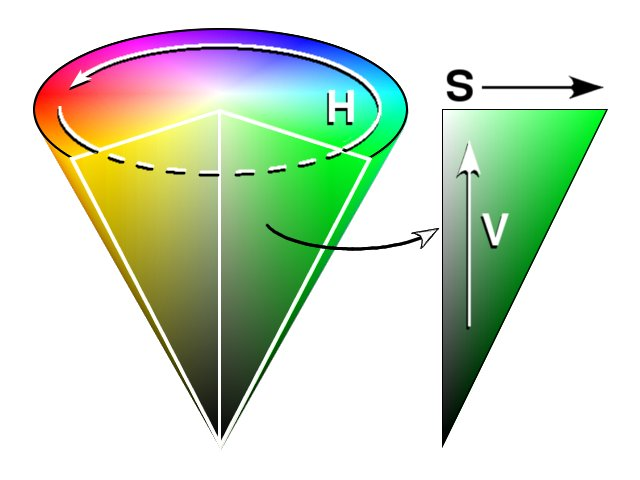
\includegraphics[scale=0.35]{HSV.jpg}
  \caption{Hue (H), ranging from 0 to 360 degrees; Saturation (S), ranging from 0 to 100\% and Value (V) ranging from 0 to 100\% }
  \label{HSV}
\end{figure}

OpenCV placed the pixels that were in the right HSV range in a new picture. This picture had a value of 1 on the pixel where our color-values were good, and a value of 0 where they were bad. This resulted in a white blob where almost every white pixel was on our object. Something like figure \ref{processed}

\begin{figure}
  \centering
      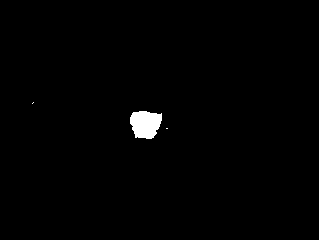
\includegraphics[scale=0.35]{processedImage.png}
  \caption{An example of our image after the first processing}
  \label{processed}
\end{figure}





\subsection{Tracking The Object}

\subsection{Picking Up The Object}

